\begin{figure}[ht]
\centering
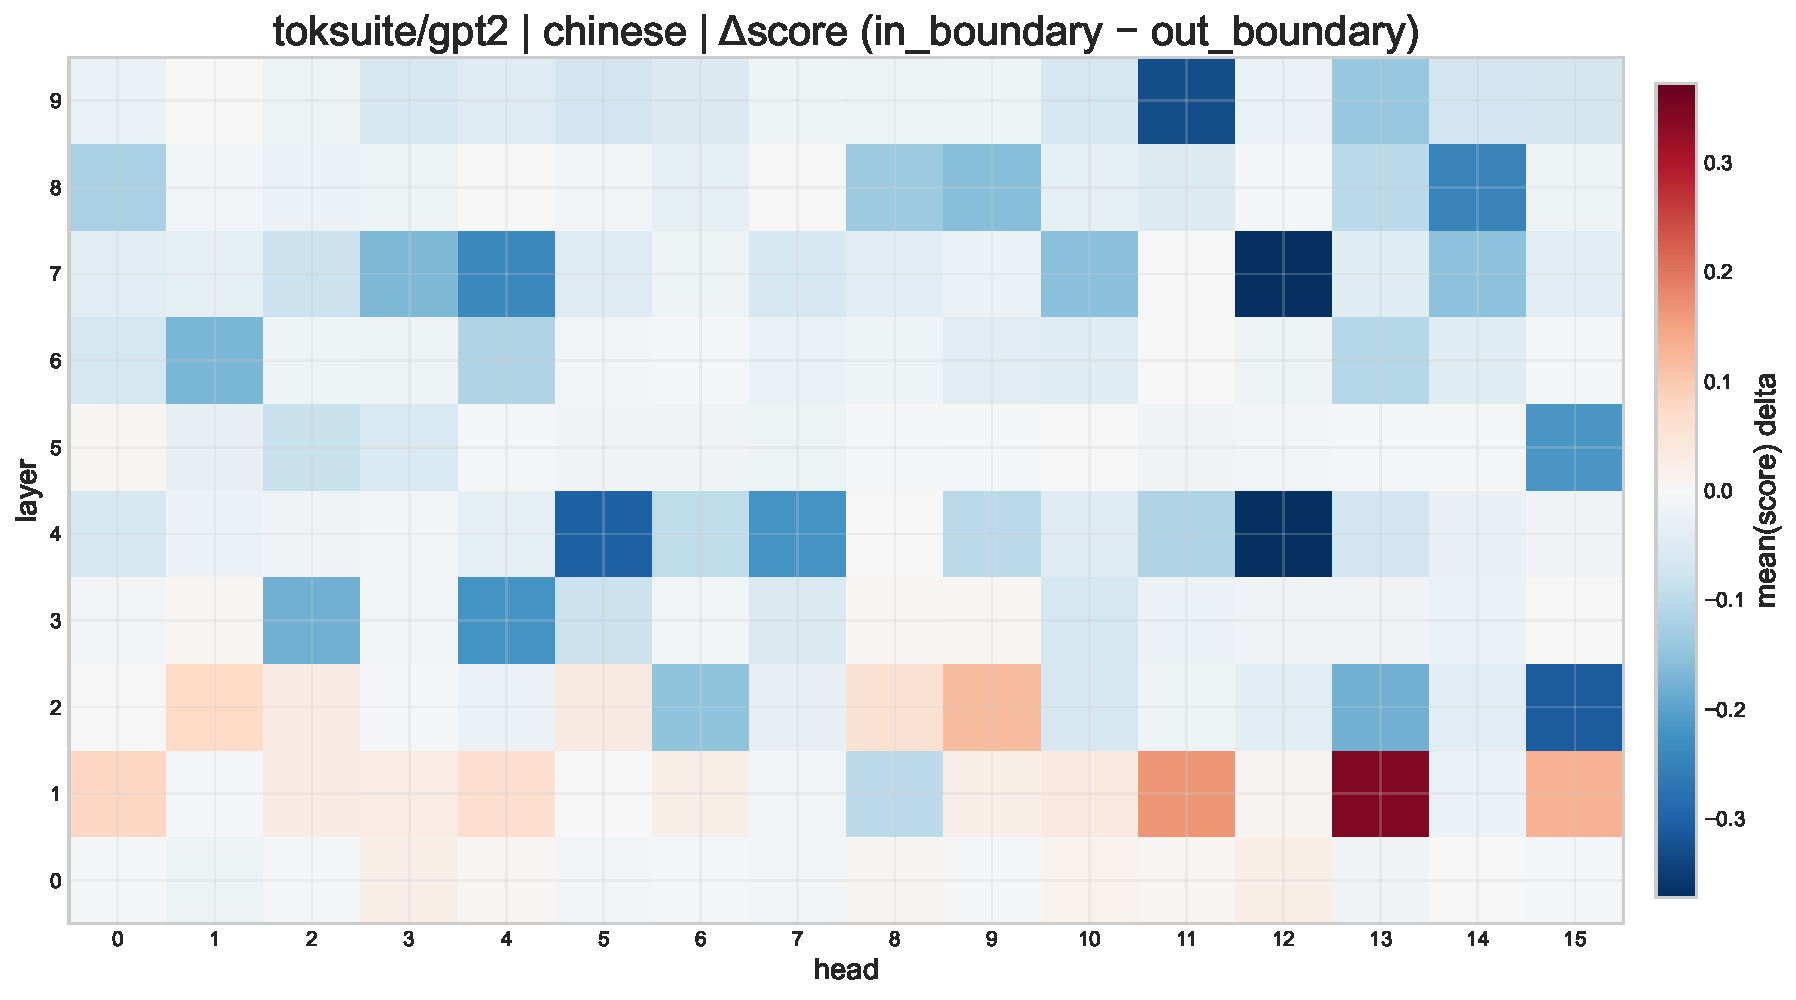
\includegraphics[width=0.5\linewidth]{plots/toksuite_gpt2_heads_deltas/heatmap_score_delta_chinese.pdf}
\caption{Heatmap showing the difference between \texttt{in\_boundary} - \texttt{out\_boundary} condition for Chinese \texttt{toksuite/gpt2}}
\label{fig:gpt2_zh}
\end{figure}

\begin{figure}[ht]
\centering
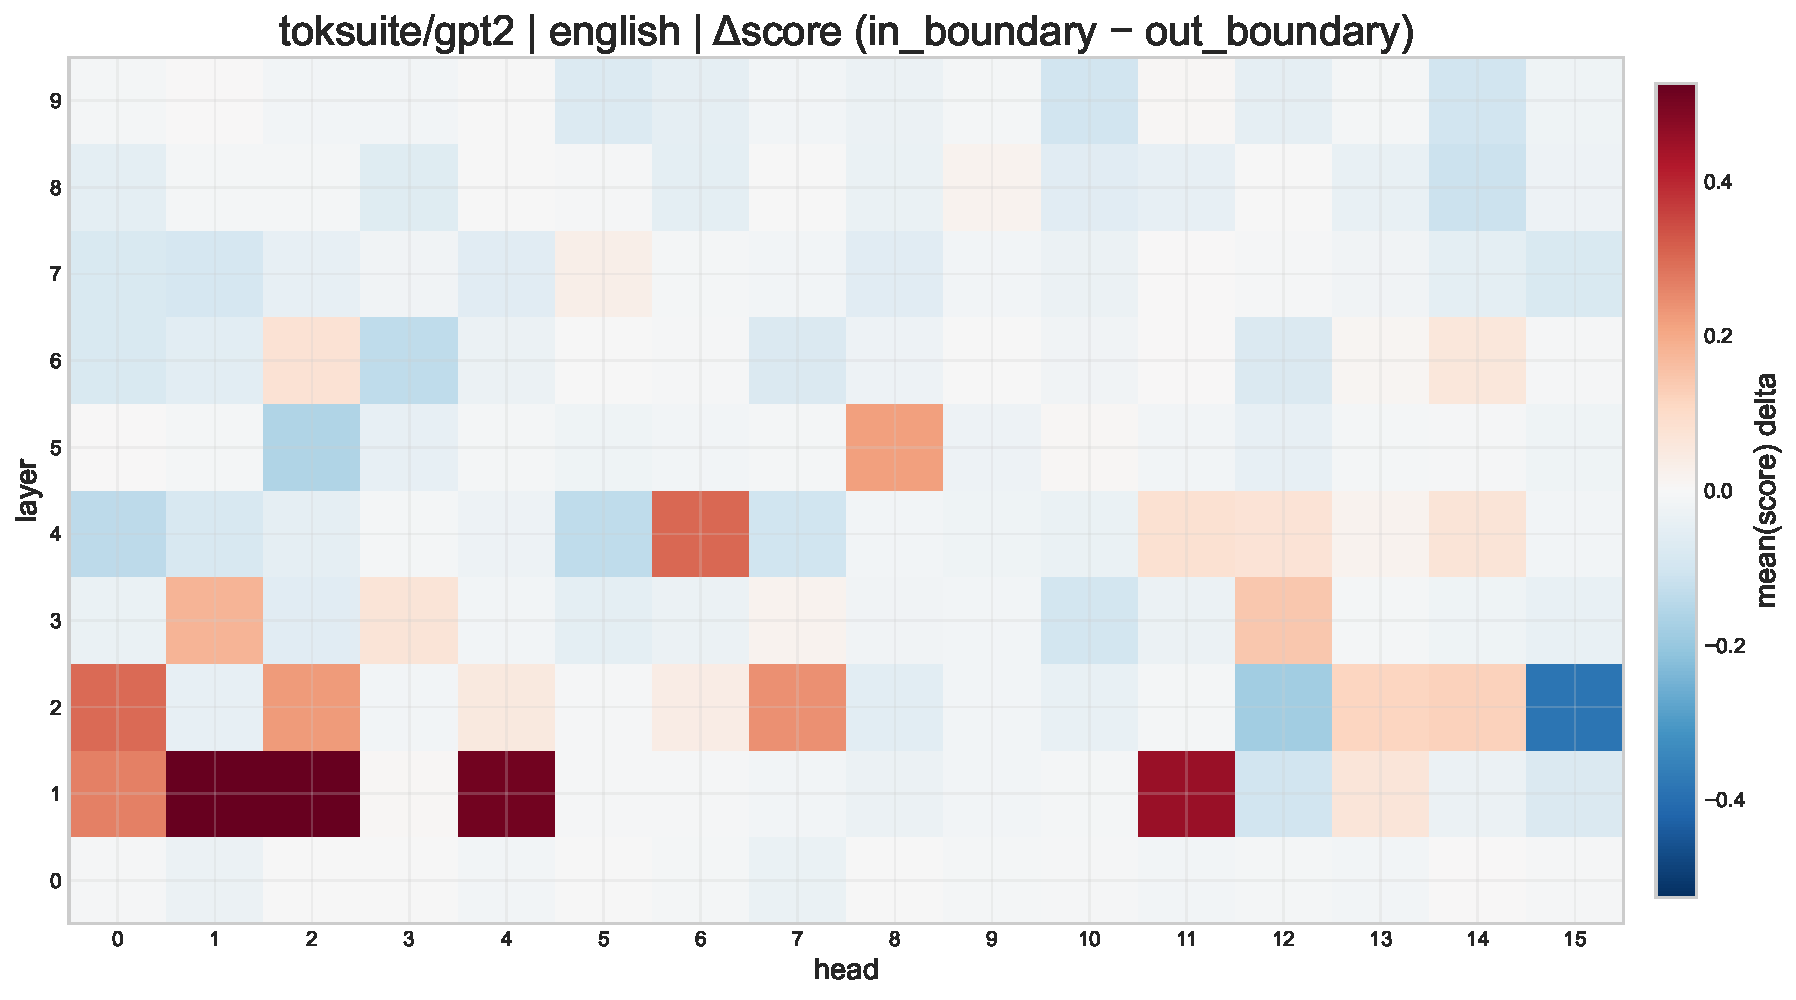
\includegraphics[width=0.5\linewidth]{plots/toksuite_gpt2_heads_deltas/heatmap_score_delta_english.pdf}
\caption{Heatmap showing the difference between \texttt{in\_boundary} - \texttt{out\_boundary} condition for English in \texttt{toksuite/gpt2}}
\label{fig:gpt2_en}
\end{figure}

\begin{figure}[ht]
\centering
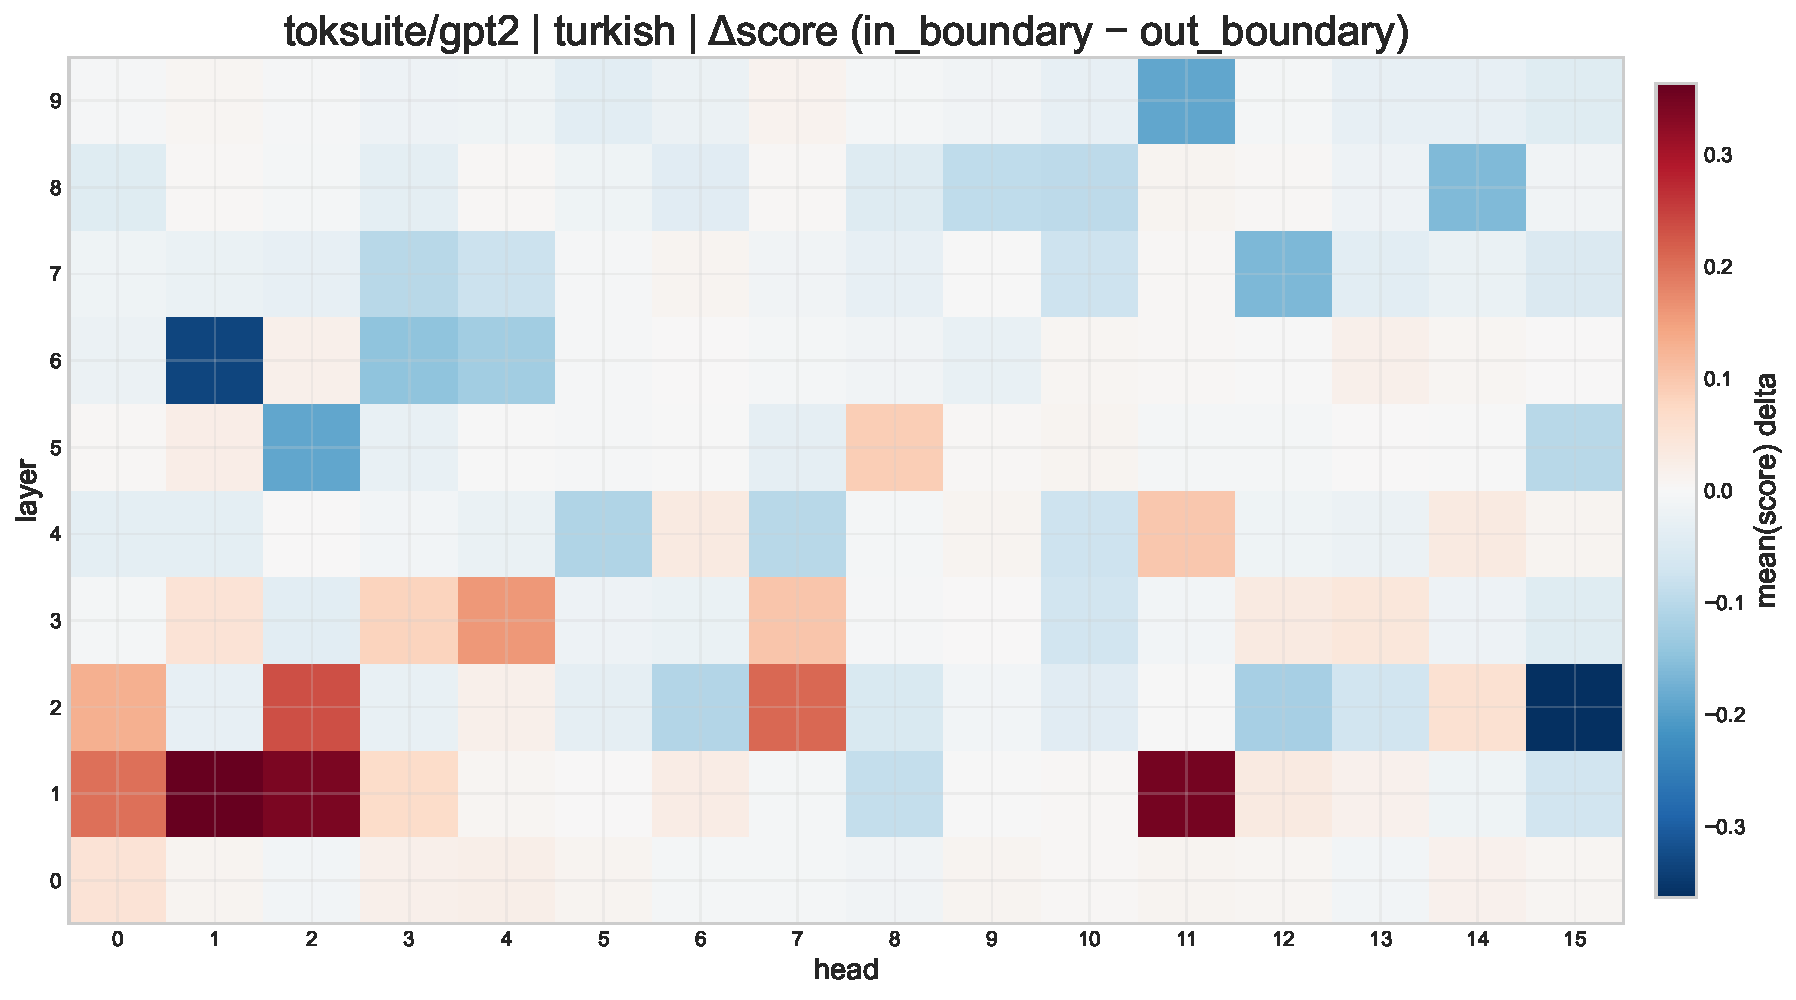
\includegraphics[width=0.5\linewidth]{plots/toksuite_gpt2_heads_deltas/heatmap_score_delta_turkish.pdf}
\caption{Heatmap showing the difference between \texttt{in\_boundary} - \texttt{out\_boundary} condition for Turkish in \texttt{toksuite/gpt2}}
\label{fig:gpt2_tr}
\end{figure}
